\section{Diagrama Entidade Relação}

O software Install\&Go é suportado por uma base de dados relacional esquematizada de acordo com as necessidades do projeto.

\begin{figure}[htb]
    \centering
    
    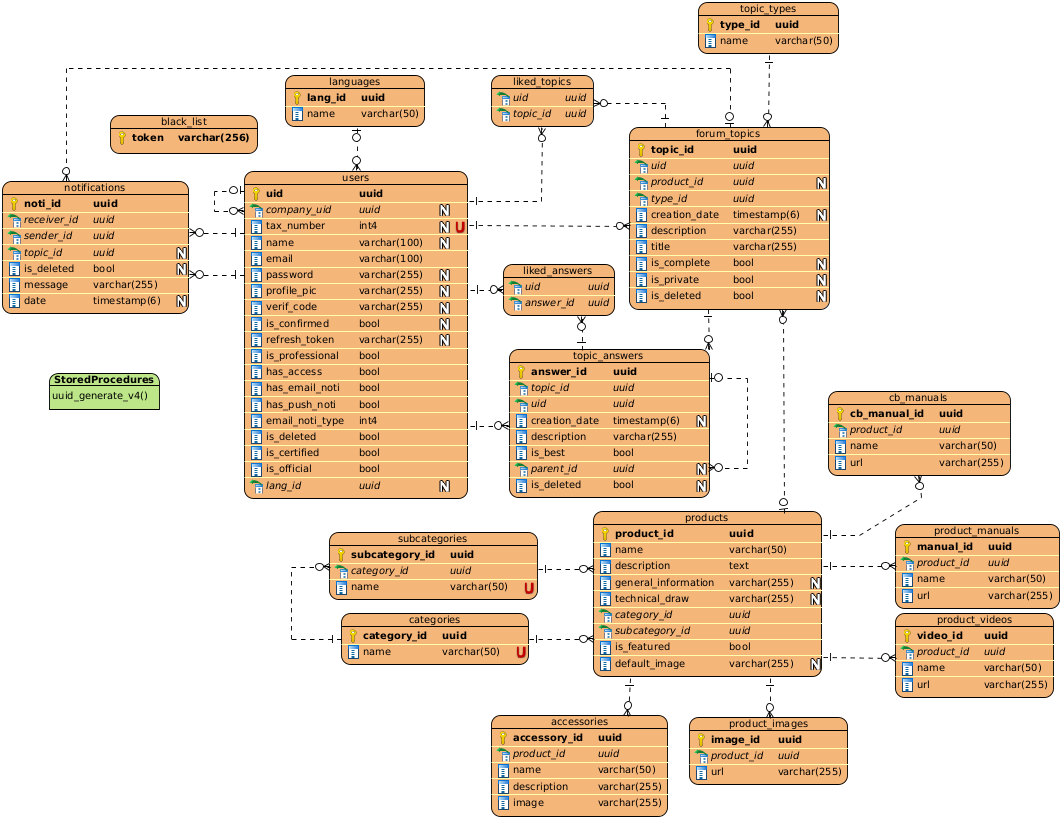
\includegraphics[width=\textwidth]{images/diagramas/diagrama_bd.png}
    \caption{Diagrama Entidade Relação base de dados Install\&Go}
    \label{fig:20}
\end{figure}

\newpage

\subsection{Escolha de diagrama de entidade relação}
Durante o desenvolvimento do diagrama de entidade relação, surgiu 
a opção de separar as empresas dos seus técnicos em duas tabelas como 
exemplificado na Figura~\ref{fig:21}. Neste sempre que se
deseja, por exemplo, obter o utilizador que criou um tópico é necessário
verificar se o \textit{uid} contido é de uma empresa ou de um técnico e apenas de seguida se obter o utilizador que criou o tópico, sendo este um exemplo entre os demais do mesmo tipo. Tendo em conta este problema foi decido optar pelo diagrama da Figura~\ref{fig:20}.

\begin{figure}[htb]
    \centering
    
    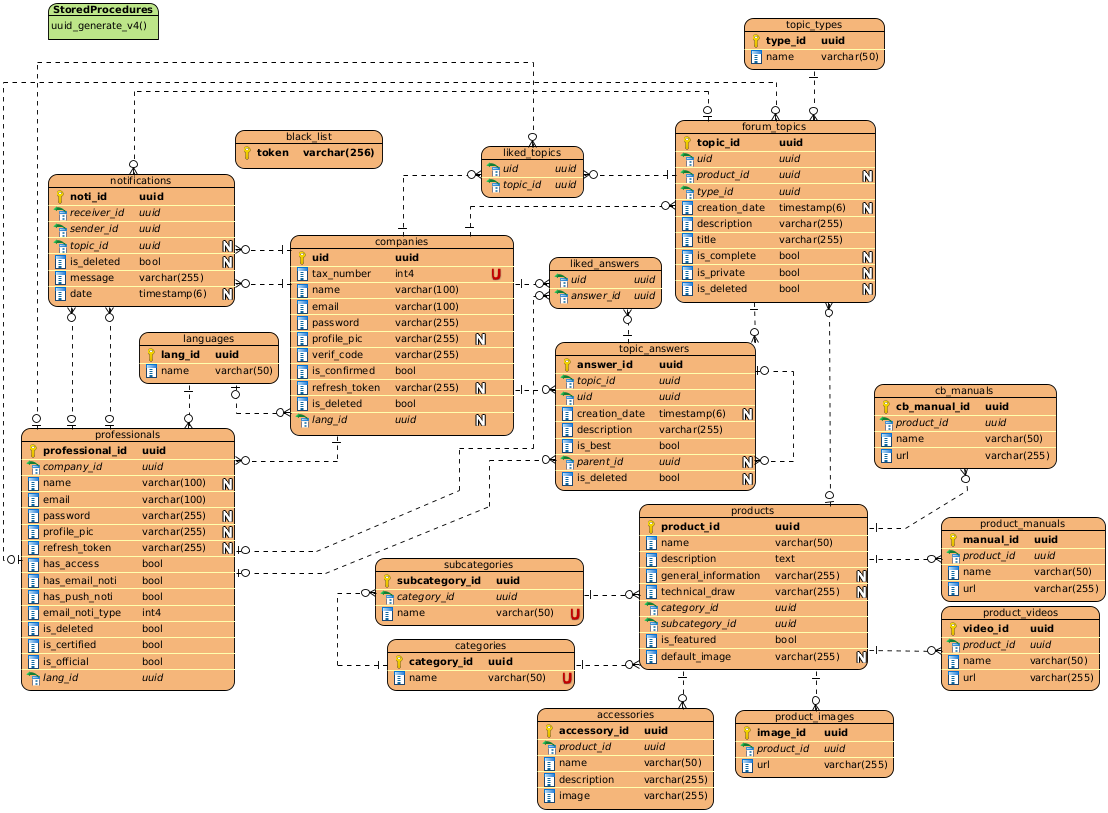
\includegraphics[width=\textwidth]{images/diagramas/diagrama_bd_alt.png}
    \caption{Diagrama Entidade Relação alternativo}
    \label{fig:21}
\end{figure}

\newpage

\subsection{Dicionário de termos}

Com intuito de alcançar o propósito de cada tabela e atributo 
foi criado um dicionário de termos para a base de dados(Tabela~\ref{tab:18}).

\definecolor{Concrete}{rgb}{0.952,0.952,0.952}
\begin{longtblr}
[
caption={Dicionário de termos da base de dados},
label={tab:22},
]{
  width = \linewidth,
  colspec = {Q[220]Q[292]Q[240]Q[215]},
  row{1} = {Concrete},
  column{1} = {c},
  cell{2}{1} = {r=19}{},
  cell{2}{2} = {r=19}{},
  cell{22}{1} = {r=2}{},
  cell{22}{2} = {r=2}{},
  cell{24}{1} = {r=2}{},
  cell{24}{2} = {r=2}{},
  cell{26}{1} = {r=2}{},
  cell{26}{2} = {r=2}{},
  cell{28}{1} = {r=7}{},
  cell{28}{2} = {r=7}{},
  cell{35}{1} = {r=10}{},
  cell{35}{2} = {r=10}{},
  cell{45}{1} = {r=8}{},
  cell{45}{2} = {r=8}{},
  cell{53}{1} = {r=2}{},
  cell{53}{2} = {r=2}{},
  cell{55}{1} = {r=3}{},
  cell{55}{2} = {r=3}{},
  cell{58}{1} = {r=4}{},
  cell{58}{2} = {r=4}{},
  cell{62}{1} = {r=8}{},
  cell{62}{2} = {r=8}{},
  cell{70}{1} = {r=4}{},
  cell{70}{2} = {r=4}{},
  cell{74}{1} = {r=4}{},
  cell{74}{2} = {r=4}{},
  vlines,
  hline{1-2,21-22,24,26,28,35,45,53,55,58,62,70,74,78} = {-}{},
  hline{3-20,23,25,27,29-34,36-44,46-52,54,56-57,59-61,63-69,71-73,75-77} = {3-4}{},
}
Tabela           & Descrição                                                                            & Atributos            & Descrição                                           \\
users            & Tabela encarregue de guardar todos os dados referentes aos utilizadores da aplicação & uid                  & Id do utilizador                                    \\
                 &                                                                                      & company\_id          & Id da empresa referente ao técnico                  \\
                 &                                                                                      & n\_contribuinte      & Número de contribuinte do utilizador                \\
                 &                                                                                      & name                 & Nome do utilizador                                  \\
                 &                                                                                      & email                & Email do utilizador                                 \\
                 &                                                                                      & password             & Password do utilizador                              \\
                 &                                                                                      & profile\_pic         & Imagem de perfil do utilizador                      \\
                 &                                                                                      & verif\_code          & Código de verificação do utilizador                 \\
                 &                                                                                      & is\_confirmed        & Verificação de se o código está confirmado          \\
                 &                                                                                      & refresh\_token       & Token de refresh                                    \\
                 &                                                                                      & is\_professional     & verificação se é profissional                       \\
                 &                                                                                      & has\_access          & verificação se tem acesso à conta                   \\
                 &                                                                                      & has\_email\_noti     & verificação se ativou notificações de email         \\
                 &                                                                                      & has\_push\_noti      & verificação se ativou notificações push             \\
                 &                                                                                      & email\_noti\_type    & tipo de notificação de email                        \\
                 &                                                                                      & push\_noti\_type     & tipo de notificação push                            \\
                 &                                                                                      & is\_deleted          & verificação se a conta se encontra apagada          \\
                 &                                                                                      & is\_certified        & verificação se é um técnico certificado             \\
                 &                                                                                      & is\_official         & verificação se é um técnico oficial                 \\
black\_list      & Tabela que guarda os tokens a bloquear                                               & token                & Token a bloquear                                    \\
liked\_topics    & Tabela encarregue de guardar todos os tópicos que foram gostados pelo utilizador     & uid                  & Id do utilizador                                    \\
                 &                                                                                      & topic\_id            & Id do tópico                                        \\
liked\_answers   & Tabela encarregue de guardar todas as respostas que receberam gosto do utilizador    & uid                  & Id do utilizador                                    \\
                 &                                                                                      & answer\_id           & Id da resposta                                      \\
topic\_types     & Tabela encarregue de guardar os tipos de tópico existentes                           & type\_id             & Id do tipo de tópico                                \\
                 &                                                                                      & name                 & nome do tipo de tópico                              \\
notifications    & Tabela encarregue de guardar todas as notificações do técnico                        & noti\_id             & Id da notificação                                   \\
                 &                                                                                      & receiver\_id         & Recetor da notificação                              \\
                 &                                                                                      & sender\_id           & Emissor da notificação                              \\
                 &                                                                                      & topic\_id            & Id do tópico em caso de estar referente a um tópico \\
                 &                                                                                      & is\_deleted          & verificação se a notificação está apagada           \\
                 &                                                                                      & message              & mensagem da notificação                             \\
                 &                                                                                      & date                 & data de emissão da notificação                      \\
forum\_topics    & Tabela encarregue de guardar todos os tópicos existentes na aplicação                & topic\_id            & Id do tópico                                        \\
                 &                                                                                      & uid                  & Id do dono do tópico                                \\
                 &                                                                                      & product\_id          & Produto referente ao tópico                         \\
                 &                                                                                      & tiype\_id            & Id do tipo referente ao tópico                      \\
                 &                                                                                      & creation\_date       & Data de criação do tópico                           \\
                 &                                                                                      & description          & Descrição do tópico                                 \\
                 &                                                                                      & title                & Titulo do tópico                                    \\
                 &                                                                                      & is\_complete         & Verificação se o tópico está finalizado             \\
                 &                                                                                      & is\_private          & Verificação se o tópico é privado                   \\
                 &                                                                                      & is\_deleted          & Verificação se o tópico está apagado                \\
topic\_answers   & Tabela encarregue de guardar todas as respostas a um tópico                          & answer\_id           & Id da resposta                                      \\
                 &                                                                                      & topic\_id            & Id do tópico                                        \\
                 &                                                                                      & uid                  & Id do dono da resposta                              \\
                 &                                                                                      & creation\_date       & Data de criação da resposta                         \\
                 &                                                                                      & description          & Descrição da resposta                               \\
                 &                                                                                      & is\_best             & Verificação se é a melhor resposta                  \\
                 &                                                                                      & parent\_id           & Id da resposta pai                                  \\
                 &                                                                                      & is\_deleted          & Verificação se o topico se encontra apagado         \\
categories       & Tabela encarregue de guardar todas as categorias de produtos existentes              & category\_id         & Id da categoria                                     \\
                 &                                                                                      & name                 & Nome da categoria                                   \\
subcategories    & Tabela encarregue de guardar as subcategorias de produtos existentes                 & subcategory\_id      & Id da subcategoria                                  \\*
                 &                                                                                      & category\_id         & Id da categoria                                     \\*
                 &                                                                                      & name                 & Nome da subcategoria                                \\*
cb\_manuals      & Tabela encarregue de guardar os manuais de utilização das placas de controlo         & cb\_manual\_id       & Id do manual                                        \\
                 &                                                                                      & product\_id          & Id do produto                                       \\
                 &                                                                                      & name                 & Nome da placa de controlo                           \\
                 &                                                                                      & url                  & Url do manual                                       \\
products         & Tabela encarregue de guardar as informações dos produtos do catálogo da empresa      & product\_id          & Id do produto                                       \\
                 &                                                                                      & name                 & Nome do produto                                     \\
                 &                                                                                      & description          & Descrição do produto                                \\
                 &                                                                                      & general\_information & Url da informação geral do produto                  \\
                 &                                                                                      & technical\_draw      & Url do desenho técnico do produto                   \\
                 &                                                                                      & category\_id         & Id da categoria de produto                          \\
                 &                                                                                      & subcategory\_id      & Id da subcategoria de produto                       \\
                 &                                                                                      & is\_featured         & Verificação se o produto é um destaque              \\
product\_manuals & Tabela encarregue de guardar os manuais de utilização dos produtos                   & cb\_manual\_id       & Id do manual                                        \\
                 &                                                                                      & product\_id          & Id do produto                                       \\
                 &                                                                                      & name                 & Nome do manual                                      \\
                 &                                                                                      & url                  & Url do manual                                       \\
product\_videos  & Tabela encarregue de guardar os videos de cada produto                               & cb\_manual\_id       & Id do video                                         \\
                 &                                                                                      & product\_id          & Id do produto                                       \\
                 &                                                                                      & name                 & Nome dao video                                      \\
                 &                                                                                      & url                  & Url do video                                        
\end{longtblr}